\documentclass{article}
\usepackage{tikz}
\usepackage[utf8]{inputenc}
\usetikzlibrary{arrows,automata}
\usepackage[all]{xy}
\usepackage{enumerate}
\usepackage{amsfonts}

\title{Práctica 4: Lenguajes Regulares}
\author{Lothar Soto Palma DNI:49079173W}
\date{\today}

\begin{document}

\maketitle

\section*{Ejercicio 1:}
Dados los alfabetos $A=\{0,1,2,3\}$ y $B=\{0,1\}$ y el homomorfismo $f$ de $A^*$ a $B^*$ dado por: $f(0)=00$, $f(1)=01$, $f(2)=10$, $f(3)=11$. Resolver las siguientes cuestiones:
\begin{enumerate}[a)]
\item Sea $L_1$ el conjunto de palabras de $B^*$ tales que acaban con la subcadena $11$. Construir un autómata finito determinista que acepte $f^{-1}(L_1)$.
\item Sea $L_3$ el conjunto de palabras de $A^*$ definido como $L_3= \{2^k3^k:1<=k<=100\}$. Construir una expresión regular que represente a $f(L_3)$.
\end{enumerate}
\textbf{Solución:}
\begin{enumerate}[a)]
\item Obtenemos la solución para para $L_1 \in B^*$:
 \begin{center}
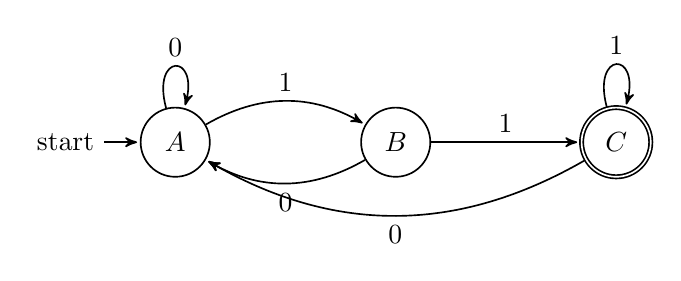
\begin{tikzpicture}[->,>=stealth',shorten >=1pt,auto,node distance=2.8cm,semithick]

	\node[state,initial]	(A)	{$A$};
	\node[state]	(B)	[right of=A] {$B$};
	\node[state,accepting] [right of=B] (C)	{$C$};

	\path (A) edge [loop above] node {$0$} (A)
		(A) edge [bend left] node {$1$} (B)
		(B) edge [bend left] node {$0$} (A)
		(B) edge node {$1$} (C)
		(C) edge [bend left] node {$0$} (A)
		(C) edge [loop above] node {$1$} (C);

\end{tikzpicture}
\end{center}
Ahora tan solo nos tenemos que fijar en que conjuntos de $A^*$ cumple que acaben en $3$:
 \begin{center}
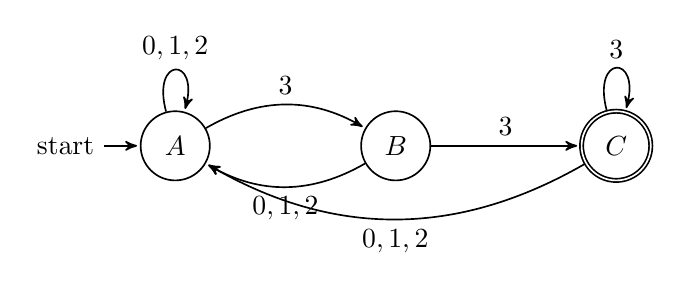
\begin{tikzpicture}[->,>=stealth',shorten >=1pt,auto,node distance=2.8cm,semithick]

	\node[state,initial]	(A)	{$A$};
	\node[state]	(B)	[right of=A] {$B$};
	\node[state,accepting] [right of=B] (C)	{$C$};

	\path (A) edge [loop above] node {$0,1,2$} (A)
		(A) edge [bend left] node {$3$} (B)
		(B) edge [bend left] node {$0,1,2$} (A)
		(B) edge node {$3$} (C)
		(C) edge [bend left] node {$0,1,2$} (A)
		(C) edge [loop above] node {$3$} (C);

\end{tikzpicture}
\end{center}
Minimizando obtenemos:
 \begin{center}
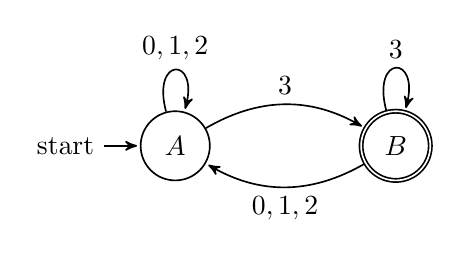
\begin{tikzpicture}[->,>=stealth',shorten >=1pt,auto,node distance=2.8cm,semithick]

	\node[state,initial]	(A)	{$A$};
	\node[state,accepting]	(B)	[right of=A] {$B$};

	\path (A) edge [loop above] node {$0,1,2$} (A)
		(A) edge [bend left] node {$3$} (B)
		(B) edge [bend left] node {$0,1,2$} (A)
		(B) edge [loop above] node {$3$} (B);

\end{tikzpicture}
\end{center}
\item $L_3\in A^*$ tiene como expresión regular $2(\epsilon+(2(\epsilon+(2(...)3))3))3$ hasta llegar a 100 veces, por lo que la expresión regular del conjunto $f(L_3)$ seria la siguiente: $10(\epsilon+(10(\epsilon+(10(...)11))11))11$. De esta manera hay el mismo número de $10$ y $11$ hasta llegar a 100. \textbf{(No pongo la expresión completa porque es ilegible)}.

\end{enumerate}

\section*{Ejercicio 2:}
Construir un autómata finito determinista que acepte el lenguaje $L_2= \{0^i1^j:i>=j\}$.\\
\textbf{Solución:}\\
Probaremos que $L_2$ no es un lenguaje regular haciendo uso del lema del bombeo:
$\forall n \in \mathbb{N},  \exists z \in L_2$ con $|z| \leq n$, $z=0^i1^j$ con $j \leq i \leq n$ tal que para toda descomposición $z=uvw$ se tiene que:
\begin{itemize}
\item $|uv| \leq n$
\item $|v| \geq 1$
\end{itemize}
Entonces podemos tomar dos casos:
\begin{itemize}
\item $u=0^i1^{j-l-k}, v=1^l, (l\geq 1), w=1^k$ y $\exists m \in \mathbb{N}$ tal que $uv^mw \not\in L_2$. Tomando $m = i+1, uv^{i+1}w = 0^i1^{j+il} \not\in L_2$.
\item $u=0^{i-s}, v=0^s1^l, (s \geq l), w=1^{j-l}$ y $\exists m \in \mathbb{N}$ tal que $uv^mw \not\in L_2$. Tomando $m = 2, uv^2w = 0^{i+s}1^{j+l} \not\in L_2$.
\end{itemize} 
Por tanto al ser un lenguaje no regular no se puede construir un autómata finito determinista que lo acepte.
\section*{Ejercicio 3:}
Minimizar si es posible el siguiente autómata usando el algoritmo visto en clase:

\begin{center}
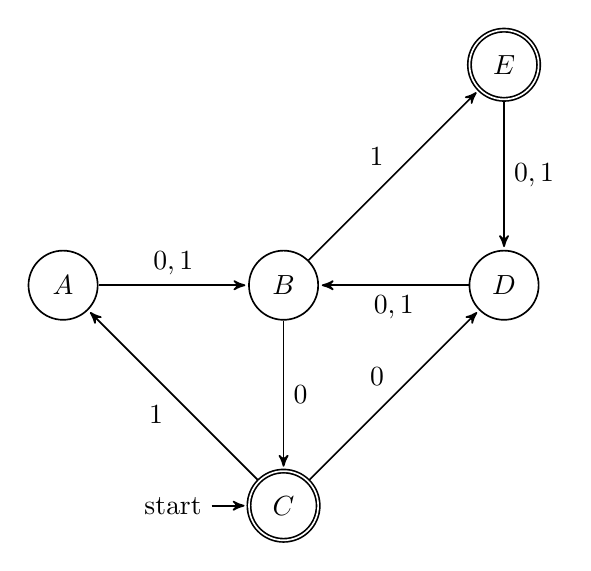
\begin{tikzpicture}[->,>=stealth',shorten >=1pt,auto,node distance=2.8cm,semithick]

	\node[state]	(A)	{$A$};
	\node[state]	(B)	[right of=A] {$B$};
	\node[state,accepting,initial] [below of=B] (C)	{$C$};
	\node[state]	(D) [right of=B]	{$D$};
	\node[state,accepting] [above of=D](E)	{$E$};

	\path (A) edge node {$0,1$} (B)
		(B) edge node {$1$} (E)
		(B) edge node {$0$} (C)
		(E) edge node {$0,1$} (D)
		(C) edge node {$0$} (D)
		(C) edge node {$1$} (A)
		(D) edge node {$0,1$} (B);

\end{tikzpicture}
\end{center}
\textbf{Solución:}\\

Comenzamos con el algoritmo, primero eliminamos los estados inaccesibles, en este caso no tenemos, ahora vemos para las parejas de estados cual de ellos tienen un camino accesible y uno de ellos es final para ello usamos esta tabla:

\begin{table}[h]
\centering
\begin{tabular}{|lllll|}
\hline
B &\multicolumn{1}{|l|}{} &  &  &  \\
 \hline
C &\multicolumn{1}{|l|}{} & \multicolumn{1}{l|}{} &  &  \\
 \hline
D &\multicolumn{1}{|l|}{}& \multicolumn{1}{l|}{} & \multicolumn{1}{|l|}{} &  \\
 \hline
E &\multicolumn{1}{|l|}{} & \multicolumn{1}{l|}{} &\multicolumn{1}{|l|}{}  & \multicolumn{1}{l|}{}\\
\hline
 & \multicolumn{1}{|l|}{A} & \multicolumn{1}{|l|}{B} & \multicolumn{1}{|l|}{C} & \multicolumn{1}{|l|}{D} \\
\hline
\end{tabular}
\end{table}

Ahora comenzamos a examinar las parejas no marcadas y calculamos el estado siguiente que se podría producir si uno de ellos está marcado lo marcamos también:\\
\newpage
\begin{table}[h]
\centering
\begin{tabular}{|lllll|}
\hline
B &\multicolumn{1}{|l|}{} &  &  &  \\
 \hline
C &\multicolumn{1}{|l|}{X} & \multicolumn{1}{l|}{X} &  &  \\
 \hline
D &\multicolumn{1}{|l|}{}& \multicolumn{1}{l|}{} & \multicolumn{1}{|l|}{X} &  \\
 \hline
E &\multicolumn{1}{|l|}{X} & \multicolumn{1}{l|}{X} &\multicolumn{1}{|l|}{}  & \multicolumn{1}{l|}{X}\\
\hline
 & \multicolumn{1}{|l|}{A} & \multicolumn{1}{|l|}{B} & \multicolumn{1}{|l|}{C} & \multicolumn{1}{|l|}{D} \\
\hline
\end{tabular}
\end{table}
Tomamos la pareja $B, A$ y miramos que estados generan:

\begin{table}[h]
\centering
\begin{tabular}{|l|l|l|}
\hline
& 0 & 1 \\
\hline
B & C & E \\
\hline
A & B & B \\
 \hline
\end{tabular}
\end{table}

Ya que $B, C$ y $B, E$ están marcados, marcamos $B, A$:\\\\

\begin{table}[h]
\centering
\begin{tabular}{|lllll|}
\hline
B &\multicolumn{1}{|l|}{X} &  &  &  \\
 \hline
C &\multicolumn{1}{|l|}{X} & \multicolumn{1}{l|}{X} &  &  \\
 \hline
D &\multicolumn{1}{|l|}{}& \multicolumn{1}{l|}{} & \multicolumn{1}{|l|}{X} &  \\
 \hline
E &\multicolumn{1}{|l|}{X} & \multicolumn{1}{l|}{X} &\multicolumn{1}{|l|}{}  & \multicolumn{1}{l|}{X}\\
\hline
 & \multicolumn{1}{|l|}{A} & \multicolumn{1}{|l|}{B} & \multicolumn{1}{|l|}{C} & \multicolumn{1}{|l|}{D} \\
\hline
\end{tabular}
\end{table}

Ahora repetimos el mismo proceso con el resto de parejas de estados sin marcar:

\begin{table}[h]
\centering
\begin{tabular}{|l|l|l|}
\hline
& 0 & 1 \\
\hline
D & B & B \\
\hline
A & B & B \\
 \hline
\end{tabular}
\begin{tabular}{|l|l|l|}
\hline
& 0 & 1 \\
\hline
D & B & B \\
\hline
B & C & E \\
 \hline
\end{tabular}
\begin{tabular}{|l|l|l|}
\hline
& 0 & 1 \\
\hline
E & D & D \\
\hline
C & D & A \\
 \hline
\end{tabular}
\end{table}
\newpage
Por último obtenemos lo siguiente:

\begin{table}[h]
\centering
\begin{tabular}{|lllll|}
\hline
B &\multicolumn{1}{|l|}{X} &  &  &  \\
 \hline
C &\multicolumn{1}{|l|}{X} & \multicolumn{1}{l|}{X} &  &  \\
 \hline
D &\multicolumn{1}{|l|}{}& \multicolumn{1}{l|}{X} & \multicolumn{1}{|l|}{X} &  \\
 \hline
E &\multicolumn{1}{|l|}{X} & \multicolumn{1}{l|}{X} &\multicolumn{1}{|l|}{}  & \multicolumn{1}{l|}{X}\\
\hline
 & \multicolumn{1}{|l|}{A} & \multicolumn{1}{|l|}{B} & \multicolumn{1}{|l|}{C} & \multicolumn{1}{|l|}{D} \\
\hline
\end{tabular}
\end{table}
Y por tanto se obtiene que $A\equiv D$ y $C\equiv E$:\\
\begin{center}
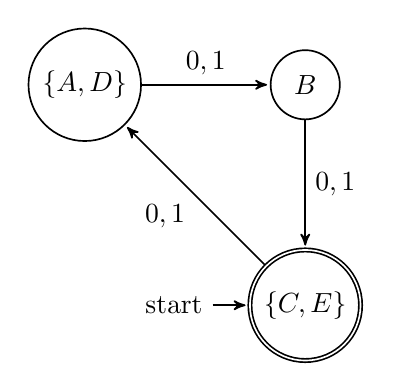
\begin{tikzpicture}[->,>=stealth',shorten >=1pt,auto,node distance=2.8cm,semithick]

	\node[state]	(A)	{$\{A,D\}$};
	\node[state]	(B)	[right of=A] {$B$};
	\node[state,accepting,initial] [below of=B] (C)	{$\{C,E\}$};

	\path (A) edge node {$0,1$} (B)
		(B) edge node {$0,1$} (C)
		(C) edge node {$0,1$} (A);

\end{tikzpicture}
\end{center}
\end{document}


